\documentclass[10pt,slidestop]{beamer}
\synctex=1

\usepackage[T1]{fontenc}
\usepackage{amsmath,amssymb,amsopn}
\usepackage{mathtools}
\usepackage{booktabs}
\usepackage{array}
\usepackage{listings}
\usepackage{matlab-prettifier}
\usepackage{xcolor}
\usepackage{tikz}
\usetikzlibrary{arrows.meta,positioning,calc,shapes.geometric}
\usepackage{algorithm}
\usepackage{algpseudocode}
\usepackage{ccicons}

\setlength{\parindent}{0pt}
\pdfcompresslevel=9

\definecolor{eclipseBlue}{RGB}{42,0,255}
\definecolor{eclipseGreen}{RGB}{63,127,95}
\definecolor{eclipsePurple}{RGB}{127,0,85}
\definecolor{codebg}{gray}{0.96}
\definecolor{darkblue}{RGB}{0,51,102}
\definecolor{darkgreen}{RGB}{0,102,51}
\definecolor{darkred}{RGB}{153,0,0}
\definecolor{lightblue}{RGB}{225,235,248}
\definecolor{lightgreen}{RGB}{223,242,223}

\lstset{
  basicstyle=\footnotesize\ttfamily,
  backgroundcolor=\color{codebg},
  frame=single,
  framesep=4pt,
  breaklines=true,
  showstringspaces=false,
  keywordstyle=\color{eclipsePurple}\bfseries,
  commentstyle=\color{eclipseGreen},
  stringstyle=\color{eclipseBlue},
}
\lstdefinestyle{ml}{style=Matlab-editor,basicstyle=\scriptsize\mlttfamily}

\setbeamertemplate{navigation symbols}{}
\setbeamertemplate{footline}{%
  \hfill\vspace*{1pt}\href{https://creativecommons.org/publicdomain/zero/1.0/}{\cczero}\hspace{.1cm}%
  \texttt{ast}\enspace--\enspace\insertframenumber/\inserttotalframenumber\enspace--\enspace\today\enspace}
\setbeamertemplate{blocks}[rounded][shadow=true]

\newcommand{\code}[1]{\texttt{#1}}
\newcommand{\ra}{$\rightarrow$}

\title{The \texttt{ast} engine}
\subtitle{Parsing, algebra and differentiation of model equations}
\author{\texttt{stephane.adjemian@univ-lemans.fr}}
\date{modBuilder technical note --- \today}

\begin{document}

\begin{frame}\titlepage\end{frame}

\begin{frame}\frametitle{Outline}\tableofcontents\end{frame}

%==============================================================================
\section{What the AST is for}
%==============================================================================

\begin{frame}\frametitle{Motivation}
  \begin{itemize}
  \item A modBuilder equation is a \textbf{string}. Strings do not compose:
    substituting \code{mc} by \code{w/mpl} in \code{a*mc\^{}2} with
    \code{strrep} gives \code{a*w/mpl\^{}2}, precedence lost.\newline
  \item The \code{ast} class parses a string into a \textbf{tree of typed
    nodes} on which every symbolic operation is defined structurally:
    static reduction, substitution, renaming, evaluation, differentiation,
    LaTeX rendering, and closed-form solving.\newline
  \item It is a \textbf{value class}: every transformation returns a new tree,
    the receiver is never mutated.\newline
  \item It is the substrate the rest of modBuilder stands on --- the steady-state
    planner, the FOC engine, the LaTeX reporters and the equation editors all
    call into it.
  \end{itemize}
\end{frame}

\begin{frame}\frametitle{Seven node types}
  Every node carries a \code{type}, a \code{value} whose shape depends on the
  type, and a \code{children} cell array.

  \medskip
  \begin{center}\scriptsize
  \begin{tabular}{@{}llll@{}}
    \toprule
    \code{type} & purpose & \code{value} & \code{children} \\
    \midrule
    \code{num}    & numeric literal & double & \code{\{\}} \\
    \code{sym}    & bare symbol (current period) & name & \code{\{\}} \\
    \code{tsym}   & lead/lag of a variable & \code{\{name,lag\}} & \code{\{\}} \\
    \code{ss}     & steady-state operator & \code{[]} & \code{\{arg\}} \\
    \code{call}   & built-in function call & fname & \code{\{arg$_1$,\dots\}} \\
    \code{binop}  & binary $+\ -\ *\ /\ \wedge$ & op & \code{\{L,R\}} \\
    \code{uminus} & unary minus & \code{[]} & \code{\{operand\}} \\
    \bottomrule
  \end{tabular}
  \end{center}

  \medskip
  \begin{itemize}
  \item Leaves: \code{num}, \code{sym}, \code{tsym}. The rest are internal.\newline
  \item \code{ss} is unary: \code{STEADY\_STATE(k/y)} is a constant w.r.t. the
    dynamics but still references \code{k} and \code{y}.\newline
  \item A subscript of zero (\code{x(0)}) collapses to a bare \code{sym} at parse
    time, so \code{x(0)} and \code{x} compare equal.
  \end{itemize}
\end{frame}

%==============================================================================
\section{Parsing}
%==============================================================================

\begin{frame}[fragile]\frametitle{Grammar}
  A small, unambiguous LL(1) expression language:

\begin{lstlisting}[language={},basicstyle=\scriptsize\ttfamily]
expr  ::= expr '+' term | expr '-' term | term
term  ::= term '*' unary | term '/' unary | unary
unary ::= '-' unary | '+' unary | power
power ::= atom '^' unary | atom
atom  ::= NUMBER | SYMBOL | SYMBOL '(' signed_int ')'
        | FNAME '(' expr (',' expr)* ')'
        | 'STEADY_STATE' '(' expr ')' | '(' expr ')'
\end{lstlisting}

  \begin{itemize}
  \item Precedence, low to high: $+\,-\ \prec\ *\,/\ \prec$ unary $-\ \prec\ \wedge$
    (right-associative). Standard, and Dynare's.\newline
  \item One token of lookahead $\Rightarrow$ recursive descent, no backtracking.\newline
  \item Disambiguation is by \textbf{name}: an identifier in
    \code{ast.RESERVED\_FNAMES} is a \code{call}; \code{STEADY\_STATE} is an
    \code{ss}; any other identifier followed by \code{(} expects a signed integer
    subscript.
  \end{itemize}
\end{frame}

\begin{frame}[fragile]\frametitle{Tokeniser and recursive descent}
  \code{ast.tokenise} scans left to right into a flat token list
  (\code{number}, \code{symbol}, parens, operators, comma). One method per
  grammar non-terminal, each a loop over its operators:

\begin{lstlisting}[language={},basicstyle=\scriptsize\ttfamily]
function [node,pos] = parse_expr(tokens,pos)
  [node,pos] = parse_term(tokens,pos);
  while tokens{pos}.type in {plus,minus}
    op = tokens{pos}.value; pos = pos+1;
    [right,pos] = parse_term(tokens,pos);
    node = ast('binop', op, {node,right});   % left-associative
  end
\end{lstlisting}

  \begin{itemize}
  \item \code{parse\_power} recurses on its right arm (right-associativity);
    the additive/multiplicative levels iterate (left-associativity).\newline
  \item The constructor \code{ast(string)} runs \code{tokenise} then
    \code{parse\_expr}. \code{ast(type,value,children)} builds one node directly.
  \end{itemize}
\end{frame}

\begin{frame}[fragile]\frametitle{\texttt{staticise}: collapsing time}
  The static version of an equation replaces every \code{tsym} by a plain
  \code{sym} --- one recursive line:

\begin{lstlisting}[style=ml]
function o = staticise(o)
  if strcmp(o.type,'tsym')
    o = ast('sym', o.value{1}, {});
  else
    for i = 1:numel(o.children)
      o.children{i} = o.children{i}.staticise();
    end
  end
\end{lstlisting}

  After this, \code{Consumption(-1)} and \code{Consumption(+1)} are the same
  node. Static residuals are what the matching, the cancellation test and the
  steady-state recognisers all work on --- name equality being unaffected by
  the lag, the static dependency structure is the same one would get by
  staticising first.
\end{frame}

%==============================================================================
\section{The algebraic engine}
%==============================================================================

\begin{frame}\frametitle{Two problems, one normal form}
  \begin{itemize}
  \item \textbf{Structural equality} (\code{ast\_equal}) is syntactic: it sees
    \code{a*b - a*b} but not \code{a*b - b*a}.\newline
  \item Almost every symbolic task needs the semantic notion --- ``are these the
    same expression?'' --- for cancellation, matching, and recogniser guards.\newline
  \end{itemize}

  \begin{block}{The device}
    \code{canonicalise} rewrites structurally equivalent trees to one shape, so
    that \code{ast\_equal} on the canonical forms captures semantic equality.
    \code{simplify} then iterates canonicalisation with local rewrite rules to a
    fixed point.
  \end{block}

  \medskip
  Pipeline: \quad\code{parse} \ra\ \code{canonicalise} \ra\ \code{simplify}
  \ra\ output, with \code{ast\_equal} now seeing commutative equivalence.
\end{frame}

\begin{frame}\frametitle{\texttt{canonicalise}}
  \begin{enumerate}
  \item Canonicalise children first (bottom-up).\newline
  \item $a - b \to a + (-b)$; \; $a / b \to a \cdot b^{-1}$; \; $--x \to x$.
    (Helpers \code{negate}/\code{invert} avoid building
    \code{uminus(uminus)} or $(b^{-1})^{-1}$.)\newline
  \item For a commutative operator ($+$ or $\cdot$):
    \begin{itemize}
    \item[a.] \textbf{flatten} the chain to an operand list --- pushing
      $-(a{+}b{+}c)$ to $[-a,-b,-c]$ and $(abc)^{-1}$ to
      $[a^{-1},b^{-1},c^{-1}]$;
    \item[b.] \textbf{cancel\_pairs}: drop $(x,-x)$ in a sum, $(x,x^{-1})$ in a
      product;
    \item[c.] \textbf{collect\_like\_terms} ($+$): decompose each term as
      $\text{coef}\cdot\text{monomial}$, group by monomial, sum coefficients;
    \item[d.] \textbf{collect\_powers} ($\cdot$): group by base, sum exponents
      (bare $f$ is $f^1$); bases matched modulo sign for integer exponents;
    \item[e.] \textbf{sort} by a stable key, rebuild left-associated.
    \end{itemize}
  \end{enumerate}
  Empty list \ra\ $0$ (sum) or $1$ (product); singleton \ra\ that operand.
\end{frame}

\begin{frame}\frametitle{The sort key and what canonical form buys}
  \begin{itemize}
  \item \code{sort\_key} orders operands: numbers $\prec$ symbols $\prec$
    steady-state $\prec$ negations $\prec$ calls $\prec$ compound binops. Stable,
    so the canonical tree is a deterministic function of the expression.\newline
  \item Consequences, all free once the tree is canonical:
    \begin{itemize}
    \item[--] $a b - b a \to 0$, $a + b - a \to b$, $(abc)/(ac) \to b$;
    \item[--] \code{ast\_equal} on canonical forms $=$ semantic equality;
    \item[--] the renderer prints $a + (-b)$ as $a - b$ and $a\cdot b^{-1}$ as
      $\tfrac{a}{b}$, so canonical internal form stays readable output.
    \end{itemize}
  \end{itemize}

  \begin{alertblock}{Cost note}
    Sorting is $O(n\log n)$ per chain; the collect passes are $O(n^2)$ in the
    operand list. Negligible per equation, but \code{canonicalise} is the hot
    path of the whole toolbox (see the performance section).
  \end{alertblock}
\end{frame}

\begin{frame}\frametitle{\texttt{simplify}: rules to a fixed point}
  Alternate \code{canonicalise} with one bottom-up rule pass until the sort key
  stops changing (capped at 64 iterations as an oscillation backstop):

  \smallskip
  \begin{itemize}\footnotesize
  \item constant folding \; $2+3\to5$, \; $6/2\to3$;
  \item identities \; $0{+}f\to f$, \; $1\cdot f\to f$, \; $f^0\to1$, \;
    $f^1\to f$, \; $1^f\to1$;
  \item structural cancellation \; $f-f\to0$, \; $f/f\to1$, \;
    $f\cdot f^{-1}\to1$;
  \item coefficient combination \; $2f + 3f \to 5f$;
    exponent combination \; $f^m f^n \to f^{m+n}$;
  \item double negation, sign propagation \; $(-1)f\to-f$, \; $f(-g)\to-(fg)$;
  \item power towers \; $(f^a)^b\to f^{ab}$ (guarded for even $a$, non-integer
    $b$; sign of $(-f)^n$ pulled out for integer $n$).
  \end{itemize}

  \smallskip
  \textbf{Local by design}: it does \emph{not} distribute, expand powers of
  sums, or put over a common denominator. Those are separate passes.
\end{frame}

\begin{frame}\frametitle{\texttt{expand} and \texttt{factor}}
  Two passes on the canonical form, opposite directions:

  \begin{columns}[t]
  \begin{column}{0.5\textwidth}
    \textbf{expand} --- distribute, unroll
    \begin{itemize}\small
    \item $a(b+c)\to ab+ac$
    \item $(a{+}b)(c{+}d)\to ac{+}ad{+}bc{+}bd$
    \item $(a_1{+}\dots{+}a_k)^n$ via the \textbf{multinomial theorem} directly
      --- only the distinct terms, each with its coefficient, no
      collect-afterwards.
    \end{itemize}
    \smallskip
    Grows the tree: a power of a $k$-term sum \ra\ $\binom{n+k-1}{k-1}$ terms.
  \end{column}
  \begin{column}{0.5\textwidth}
    \textbf{factor} --- pull out a common factor
    \begin{itemize}\small
    \item $ab+ac\to a(b+c)$
    \item $a/b+c/b\to (a+c)/b$
    \item $4ab+6ac\to 2a(2b+3c)$
    \end{itemize}
    \smallskip
    Multiset intersection of the per-term factor lists; numeric GCD when all
    coefficients are integers. Shrinks (or preserves) size. Does not yet reason
    about power identities ($a^2+a^3$).
  \end{column}
  \end{columns}

  \medskip
  These two, iterated under \code{complexity}, are how the linearisation
  coefficients are put into their most readable form.
\end{frame}

%==============================================================================
\section{Rewriting equations}
%==============================================================================

\begin{frame}\frametitle{Three ways to rewrite}
  \begin{block}{\texttt{substitute(name, repl [, params])} --- lag-aware}
    Replace every \code{sym(name)} and \code{tsym(name,k)} by \code{repl}, the
    replacement \textbf{shifted by $k$}. Substituting \code{mc} by \code{w/mpl}
    into \code{pi - beta*mc(-1)} gives \code{pi - beta*(w(-1)/mpl(-1))}.
    \code{params} names the time-invariant symbols kept unshifted;
    \code{STEADY\_STATE} leaves never shift.
  \end{block}
  \begin{block}{\texttt{replace\_subtree(target, repl)} --- structural}
    Replace every subtree \emph{equal} to \code{target} (both canonicalised, so
    \code{a*b} matches \code{b*a}). Literal --- no lag shift. The right tool when
    the target is an expression, not a symbol.
  \end{block}
  \begin{block}{\texttt{rename(old, new)} --- relabel}
    Swap a name in \code{sym}/\code{tsym}/\code{ss}, preserving lag and
    steady-state wrapping. Function names untouched.
  \end{block}
  \code{modBuilder.subs} dispatches: \code{substitute} for a symbol target,
  \code{replace\_subtree} for an expression target.
\end{frame}

%==============================================================================
\section{Differentiation}
%==============================================================================

\begin{frame}\frametitle{\texttt{diff\_ast(name [, lag])}}
  Symbolic $\partial/\partial\,\text{name}(\text{lag})$, returned simplified.

  \begin{itemize}
  \item \textbf{Period-specific}. With \code{lag=0}, only bare \code{sym(name)}
    differentiate; \code{K(-1)} is an independent variable, so
    \code{ast('K(-1)').diff\_ast('K')} $=0$. Pass the lag, or \code{staticise}
    first for all-periods (steady-state) semantics.\newline
  \item \code{ss} nodes are constants \ra\ $0$.\newline
  \item The $\wedge$ rule branches on which arm depends on the target:
    $u^n$, $a^v$, general $u^v$. Functions by the chain rule.\newline
  \item \textbf{24 function rules}: \code{log}, \code{exp}, \code{sqrt},
    \code{cbrt}, the six trig and six hyperbolic and their inverses,
    \code{normcdf}, \code{normpdf}, \code{erf}, and the sub-gradient conventions
    for \code{abs}, \code{sign}, \code{min}, \code{max}
    ($\max(u,v)=\tfrac{u+v+|u-v|}{2}$).\newline
  \item Only the time-series operators \code{diff}, \code{adl},
    \code{EXPECTATION} lack a rule \ra\ \code{ast:diff\_ast:noRule}, the signal
    for a solver to fall back to automatic differentiation.
  \end{itemize}
\end{frame}

%==============================================================================
\section{Solving for a symbol}
%==============================================================================

\begin{frame}\frametitle{\texttt{isolate(x)}: closed form of $t = 0$ for $x$}
  Reads $t$ as the residual $\text{LHS}-\text{RHS}$; returns \code{rhs} with
  $x=\text{rhs}$, or \code{[]}. Canonicalise, simplify, then four recognisers
  in order:

  \begin{enumerate}
  \item \textbf{invertible call} --- \code{exp}/\code{log} wrapping $x$, recurse
    on the inverted equation. Several copies of the \emph{same} call are summed,
    so $\log Z - \rho\log Z(-1) - e$ closes to $Z = \exp(e/(1-\rho))$;
  \item \textbf{linear} \; $a x + b = 0$;
  \item \textbf{monomial} \; $a x^d + b = 0$;
  \item \textbf{binomial power} \; $c_p x^p + c_q x^q = 0 \Rightarrow
    x=(-c_q/c_p)^{1/(p-q)}$.
  \end{enumerate}

  \smallskip
  If all fail and $x$ sits under a denominator, multiply through (sound under the
  non-zero steady-state convention) and retry once.

  \smallskip
  \textbf{Steady-state semantics}: $x$ and its leads/lags are one unknown and are
  aggregated; other variables keep their lead/lag structure.
\end{frame}

\begin{frame}\frametitle{\texttt{isolate}: the diagnostics it returns}
  The second output \code{info} is what lets the planner tell three kinds of
  failure apart:

  \begin{itemize}
  \item \code{info.unit\_root} --- every $x$-term matched the same call $f(P)$
    but the summed coefficient folded to $0$: the equation pins the
    \textbf{growth} of $f(P)$, not its level. (Surfaces as the planner's
    unit-root warning.)\newline
  \item \code{info.coefs} --- the pinning divisors along the successful chain,
    symbolically non-zero by construction. A caller holding a calibration
    evaluates them to catch \textbf{knife-edge} points where the closed form
    divides by a numerical zero ($1-R$ at $R=1$).\newline
  \item \code{[]} with neither flag --- the pattern is simply none of the four.
  \end{itemize}

  \smallskip
  Used to close singleton steady-state blocks, and by \code{eliminate} to
  substitute an auxiliary (e.g. a Lagrange multiplier) back out of the model.
\end{frame}

\begin{frame}\frametitle{Simultaneous linear blocks: Bareiss + Cramer}
  When a block of equations is jointly \emph{linear} in its unknowns:

  \begin{itemize}
  \item \code{linearise\_system} extracts $A\,x + b = 0$ by differentiating each
    residual w.r.t. each unknown (constant entries $\Rightarrow$ linear);\newline
  \item \code{solve\_linear\_system} solves $A x = -b$ by
    \textbf{fraction-free (Bareiss) triangulation} then back-substitution.
  \end{itemize}

  \begin{block}{Why fraction-free}
    Ordinary Gaussian elimination on symbolic entries builds nested fractions
    that explode. Bareiss (1968) keeps every intermediate a \emph{polynomial} by
    exact division by the previous pivot, so the entries stay compact. The
    determinant is $\pm U_{nn}$ read off the triangular form --- reused as the
    singularity / knife-edge probe.
  \end{block}

  Capped at size 8: the $O(n^3)$ polynomial fill-in is prohibitive beyond that,
  and the emitted assignments would be unreadable anyway.
\end{frame}

%==============================================================================
\section{Rendering}
%==============================================================================

\begin{frame}\frametitle{\texttt{to\_latex} and \texttt{complexity}}
  \code{to\_latex(map, dated)} renders the tree it is given --- it does
  \emph{not} canonicalise, so the caller controls the algebraic form.
  \begin{itemize}\small
  \item \code{tsym} \ra\ subscripts ($K(-1)\to K_{t-1}$); \code{ss} \ra\
    $\cdot^{\star}$; \code{exp} \ra\ $e^{\cdot}$; division \ra\ \code{\textbackslash frac};
  \item every product of inverse factors renders as ONE fraction
    ($E x^{-1} y^{-1} \to \frac{E}{xy}$); a lone $x^{-1}\to\frac{1}{x}$;
  \item a sum leads with a non-negated term when it has one;
  \item a base already ending in a superscript uses invisible
    \code{\textbackslash left. \textbackslash right.} to avoid a double superscript.
  \end{itemize}

  \begin{block}{\texttt{complexity}: choosing between equal forms}
    Two forms can be algebraically equal yet one reads far better. \code{complexity}
    scores the \textbf{rendering}: glyph count (each control sequence counts one,
    so naming is neutral), plus a penalty per fraction and per level of fraction
    nesting, plus one for a leading minus. \code{fraction\_stats} counts fractions
    \emph{as the renderer emits them}, not as the tree stores them. Callers
    generate candidate forms (\code{factor}, \code{expand}, \code{single\_fraction})
    and keep the argmin.
  \end{block}
\end{frame}

%==============================================================================
\section{Performance}
%==============================================================================

\begin{frame}\frametitle{Where the time goes, and the fix}
  Profiling the 13-variable core block: \textbf{$\sim$95\% of the time is in
  \code{canonicalise}} and its helpers --- 40 million calls, the overwhelming
  majority re-canonicalising a tree already in canonical form (every
  \code{simplify} fixed-point iteration, every \code{isolate} probe re-traverses
  the whole tree).

  \medskip
  Two coupled levers, both landed:
  \begin{itemize}
  \item \textbf{\code{sort\_key} memoisation} --- each node caches its structural
    key (\code{skey}), invalidated when a child changes. Prerequisite for the
    next lever.\newline
  \item \textbf{\code{canon} flag} --- a boolean per node, set when
    \code{canonicalise} reaches its fixed point and short-circuited at the top of
    the method. A node already canonical is returned untouched, pruning the
    recursive descent.
  \end{itemize}

  \smallskip
  Together they dry up the 40M redundant traversals; the memoised key makes each
  survivor cheap.
\end{frame}

%==============================================================================
\section{Consumers}
%==============================================================================

\begin{frame}\frametitle{Who calls the AST}
  \begin{center}
  \scalebox{0.95}{
  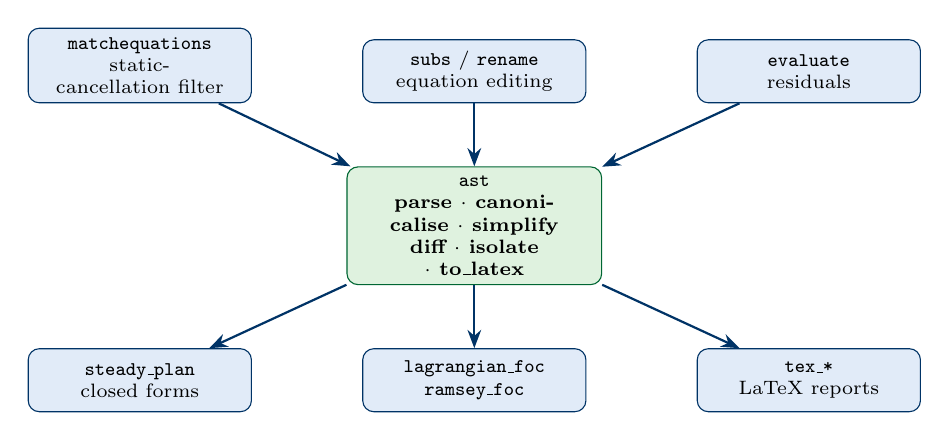
\begin{tikzpicture}[
    node distance=5mm and 7mm,
    box/.style={rectangle,draw=darkblue,fill=lightblue,rounded corners,
      align=center,minimum height=8mm,font=\scriptsize,text width=26mm},
    core/.style={rectangle,draw=darkgreen,fill=lightgreen,rounded corners,
      align=center,minimum height=9mm,font=\scriptsize\bfseries,text width=30mm},
    a/.style={-{Stealth},darkblue,thick}]
    \node[core] (ast) {\texttt{ast}\\parse $\cdot$ canonicalise $\cdot$ simplify\\diff $\cdot$ isolate $\cdot$ to\_latex};
    \node[box,above left=8mm and 12mm of ast] (match) {\texttt{matchequations}\\static-cancellation filter};
    \node[box,above=8mm of ast] (subs) {\texttt{subs} / \texttt{rename}\\equation editing};
    \node[box,above right=8mm and 12mm of ast] (eval) {\texttt{evaluate}\\residuals};
    \node[box,below left=8mm and 12mm of ast] (plan) {\texttt{steady\_plan}\\closed forms};
    \node[box,below=8mm of ast] (foc) {\texttt{lagrangian\_foc}\\ \texttt{ramsey\_foc}};
    \node[box,below right=8mm and 12mm of ast] (tex) {\texttt{tex\_*}\\LaTeX reports};
    \draw[a](match)--(ast); \draw[a](subs)--(ast); \draw[a](eval)--(ast);
    \draw[a](ast)--(plan); \draw[a](ast)--(foc); \draw[a](ast)--(tex);
  \end{tikzpicture}}
  \end{center}

  \smallskip
  The same tree, and the same handful of algebraic primitives, serve editing,
  analysis, differentiation and rendering. The steady-state deck is the largest
  consumer --- it is the subject of the companion note.
\end{frame}

\begin{frame}\frametitle{Summary}
  \begin{itemize}
  \item A value-class AST of seven node types, parsed by recursive descent.\newline
  \item \code{canonicalise} gives a normal form; \code{simplify} reaches a
    local fixed point on it; \code{expand}/\code{factor}/\code{single\_fraction}
    reshape it, \code{complexity} choosing between shapes.\newline
  \item \code{substitute} / \code{replace\_subtree} / \code{rename} rewrite;
    \code{diff\_ast} differentiates (24 rules, \code{noRule} fallback);
    \code{isolate} solves, with diagnostics; Bareiss closes linear blocks.\newline
  \item \code{to\_latex} renders any form faithfully.\newline
  \item Memoised keys and a canonical-form flag make the hot path affordable.
  \end{itemize}

  \vfill
  \centering\small Reference: \texttt{src/@ast/README.md} and the method
  docstrings in \texttt{src/@ast/ast.m}.
\end{frame}

\end{document}
